
	\section{ACM/ICPC World Finals 2012}
		\subsection{ACM/ICPC World Finals 2012 A Asteroid Rangers}
			\subsubsection{题目大意}
				三维空间上有 $N$ 个点,第 $i$ 个点在 $t$ 时刻的位置 $\mathbf{p}_i = (\mathbf{a}_i + \mathbf{v}_i t)$,其中 $\mathbf{a}_i,\mathbf{v}_i$ 为给定常向量。
				$N$ 个点两两有连边,权值为欧几里德距离。试问从 $t = 0 $时起,$N$ 个点的最小生成树会变化几次。
			
				$N \le 50$。任意时刻任意两个点不会重合。如果在 $t_0$ 时刻某棵树\emph{成为}了最小生成树,那么在接下来的 $10^{-6}$ 时间里,该树是唯一的最小生成树。初始时刻最小生成树唯一。多组询问。
			\subsubsection{算法讨论}
				考虑 Kruskal 算法求最小生成树的过程以及边权变化的连续性,显然,只有当两条边的权值相等时,才可能有新的最小生成树出现。不妨求出这些时刻,方法是解二次(可能会退化为一次或零次)方程 $\left(\mathbf{p}_u - \mathbf{p}_v\right)^2 = \left(\mathbf{p}_r - \mathbf{p}_s\right)^2$,其中 $(u,v),(r,s)$ 是正在考察的两条边。这些时间点有不超过 $2\binom{\binom{N}{2}}{2} = \mathcal{O}\left(N^4\right)$ 个。
				
				对于上面求出的每个时间 $t$,我们只需验证 $(t + \epsilon)$ 时最小生成树是否改变,此处 $\epsilon$ 可取 $\num{1e-8}$。如果改变,则答案增加一。
				
				存在一个减枝。注意到如果在 $t$ 时刻最小生成树发生改变,那么一定是将被超越的边当前正在最小生成树内,而将超越其的边目前不在最小生成树。若当前的情况不是这样,那么最小生成树肯定不会变化,可以直接忽略掉该时间点 $t$。
			\subsubsection{时空复杂度}
				时间复杂度 $\mathcal{O}\left(N^6\right)$。上述减枝的优化效果很好,实际情况远远达不到该上限。
					
				空间复杂度 $\mathcal{O}\left(N^4\right)$。
		\newpage
		\subsection{ACM/ICPC World Finals 2012 B Curvy Little Bottles}
			\subsubsection{题目大意}
				有一个瓶子,其侧面由多项式函数 $y=f(x)$ 在 $x \in \left[L,R\right]$ 上绕 $x$ 轴旋转 \SI{360}{\degree} 而成,而底部和顶部分别是半径为 $f(L), f(R)$ 的圆。试求
				\begin{enumerate}
					\item 其体积;
					\item 若每隔 $V_0$ 的体积就给瓶子贴上标签,问最底部的不超过 $k$ 个标签到瓶子底端的距离。
				\end{enumerate}
				
				多项式 $f(x)$ 的次数 $N$ 不超过 $10$。$\forall x \in \left[L,R\right], f(x) > 0$。$k = 8$。多组询问。
			\subsubsection{算法讨论}
				显然体积为 $\int_{L}^{R} \pi f(x)^2 dx$。 求出多项式 $f(x)$ 的平方的原函数 $F(x) = \int f(x)^2 dx = \sum_{i=1}^{2N+1} k_ix^i$,那么第一问体积
				\begin{align}
					\int_{L}^{R} \pi f(x)^2 dx = \pi \left(F(R) - F(L)\right)
				\end{align}
				
				第二问相当于解方程 $\pi \left(F(x) - F(L)\right) = \mathrm{C}_1$ 即 $F(x) = \mathrm{C}_2$,其中 $\mathrm{C}_1,\mathrm{C}_2$ 为常数。由于 $f(x)>0$,故 $F(x)$ 单调,使用二分法即可求解。
			\subsubsection{时空复杂度}
				单组测试时间复杂度 $\mathcal{O}\left(N^2 + k p N\right)$。$p$ 是二分时检验答案的次数,与精度相关。
					
				空间复杂度 $\mathcal{O}\left(N\right)$。
		\newpage
		\subsection{ACM/ICPC World Finals 2012 C Bus Tour}
			\subsubsection{题目大意}
				给定无向图 $G =(V,E)$,边有边权 $W : E \mapsto \mathbb{R}_+$,$V$ 中有一个源 $s$,有一个汇 $t$。请选择一个子集 $X \subset V \setminus \{ s,t\}$ 使得 $|X| = \lfloor (|V|-2)/2 \rfloor, Y = V \setminus \{ s,t\} \setminus X$,且使得路径 
				\begin{align}
					s \rightarrow X  \text{ 中的结点} \rightarrow Y \text{  中的结点} \rightarrow t \rightarrow X \text{ 中的结点}
				 \rightarrow Y \text{ 中的结点}   \rightarrow s  \label{2012cpath}
				\end{align} 的长度最小化。
				几次访问集合中的节点的先后任意,且同样的集合前后两次的顺序可以不同。 求此最小的长度。
			
				$|V| = N \le 20$。多组询问。
			\subsubsection{算法讨论}
				设 $F[p][S]$ 表示从 $s$ 出发,经过集合 $S$ 中的结点到达 $p$ 结点的最短路径长度,$G[p][S]$ 表示从 $t$ 出发,经过集合 $S$ 中的结点到达 $p$ 结点的最短路径长度。使用 Floyed 算法求出两两间的最短路后,容易使用 SCDP 求出这两个值。
				
				随后 \eqref{2012cpath} 被分为了几部分 
				\begin{align}
					p  = \; & s \rightarrow X\setminus\{p\} \rightarrow p  , p \rightarrow q , q \rightarrow Y\setminus\{q\} \rightarrow t, \notag \\ & t \rightarrow X\setminus\{u\} \rightarrow u,u\rightarrow v, v \rightarrow Y \setminus \{v\} \rightarrow s
				\intertext{对应的最短路径长度为 }
					d_p  =\;  &\min_{p\in X,q\in Y} \left(F[p][X] + d(p,q) + G[q][Y]\right)  + \notag \\ & \min_{u\in X,v\in Y} \left(G[u][X] + d(u,v) + F[v][Y]\right) 
				\end{align}
				其中 $d(\cdot,\cdot)$ 表示两点最短路长度。枚举所有的 $X,p,q,u,v$,取最小值作为答案。
				
				特殊处理 $N = 3$ 的情况。
			\subsubsection{时空复杂度}
				时间复杂度 $\mathcal{O}\left(N^22^N\right)$。
					
				空间复杂度 $\mathcal{O}\left(N2^N\right)$。
		\newpage

		\subsection{ACM/ICPC World Finals 2012 D
Fibonacci Words}
			\subsubsection{题目大意}
				设第 $i$ 个斐波纳契串为 $S(i)$,则 $S(0)=0, S(1) = 1$ 且
				\begin{align}
					S(i)=S(i-1)+S(i-2)
				\end{align}
				$+$ 表示字符串的连接。问字符串 $T$ 在 $S(N)$ 中出现了多少次。
			
				$N \le 100, |T| = M \le \num{100000}$。$|x|$ 表示字符串 $x$ 的长度。答案 $< 2^{63}$。多组询问。
			\subsubsection{算法讨论}
				动态规划,设 $F[i]$ 表示 $T$ 在 $S(i)$ 中出现的次数
				\begin{align}
					F[i] & = F[i-1] + F[i-2] + T \text{ 在 $S(i-1)$ 与 $S(i-2)$ 衔接的地方出现的次数}
				\intertext{这个衔接处出现的次数可通过将 $S(i-1)$ 长度最多不超过 $(M-1)$ 的后缀与  $S(i-2)$ 长度最多不超过 $(M-1)$ 的前缀连接起来,运行 KMP 算法求得。边界}
					F[0] &= [V = 0]\\
					F[1]& = [V = 1]
				\end{align}
			
				虽然答案保证  $< 2^{63}$,但 $|S(N)| $ 不一定低于 $2^{63}$,需要处理斐波纳契串长度溢出的问题。
			\subsubsection{时空复杂度}
				时间复杂度 $\mathcal{O}\left(NM\right)$。
					
				空间复杂度 $\mathcal{O}\left(M\right)$。
		\newpage

		\subsection{ACM/ICPC World Finals 2012 E Infiltration}
			\subsubsection{题目大意}
				求竞赛图 $G=(V, E)$ 的最小支配集。
			
				$N = |V| \le 75$。
			\subsubsection{算法讨论}
				可以构造一个大小为 $\mathcal{O}{\left(\log N\right)}$ 的解。由于是竞赛图,故总存在出度超过 $\frac{N-1}{2}$ 的点。选择该点,并将该点和它所指向的点都从原图剔除,这样原图的点数规模缩小为原来的 $\frac{1}{2}$。经过   $\mathcal{O}{\left(\log N\right)}$ 次操作后,图被删除为空图,而选出的点就是一个支配集,大小  $\mathcal{O}{\left(\log N\right)}$ 。 对于该题 $N \le 75$ 的情况,这个解的大小不超过 $6$。
				
				那么只需搜索是否存在低于上述构造解的方案。对于此题,搜索量不超过  $\binom{75}{5} = \num{17259390}$。
				
				可用位运算优化搜索过程。	
			
			\subsubsection{时空复杂度}
				时间复杂度 $\mathcal{O}\left( N ^{ \log_2 N}\right)$。
					
				空间复杂度 $\mathcal{O}\left(N^2\right)$。
		\newpage

		\subsection{ACM/ICPC World Finals 2012 F Keys}
			\subsubsection{题目大意}
				给定一些钥匙和钥匙环,有些已经套在一起。现在请通过解开钥匙(环)和将钥匙(环)套在一起的方法,将钥匙按指定的分法分给两个人,使得每个人只需拿走一串连好的钥匙环即可解决问题(如果该人需要拿钥匙)。请在最小化钥匙和钥匙环之间的捆绑(解绑)的情况下,最小化钥匙环之间的捆绑(解绑)的次数。
				
				\begin{figure}[!htb]
 					\centering
					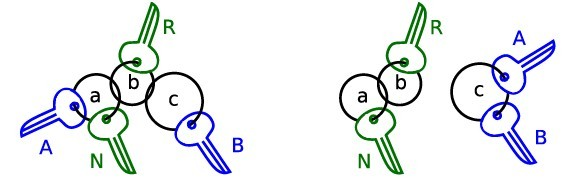
\includegraphics[width=0.8 \textwidth]{2.jpg}
					\caption{一个例子}
				\end{figure}
					
				钥匙环 $N \le 26, $ 每个人各自分配的钥匙 $ M\le 13$。钥匙串连起来只会形成森林,不会有环。


			\subsubsection{算法讨论}
				先忽略空钥匙环。如果某一个钥匙环上两个人的钥匙不等,那么一点相对较少的那个人的钥匙将被取走。如果两个钥匙串上的钥匙相等,那么两种情况都有可能,需要枚举。 这样的钥匙环的数量不会超过 $M$,故枚举只需耗费 $\mathcal{O}\left(2^M\right)$ 的时间。枚举非空钥匙串各自的主人后,只需使用树形动态规划,确定空钥匙串的分配方法,以最小化钥匙环间的操作次数。
				
				注意到如果两个人都有要拿走的钥匙,那么一定要保证两个人各自都有一个属于他的钥匙环,而上述的枚举和动态规划可能会忽略这个问题。所以再枚举一次某个人只拥有一个钥匙环的情况也是有必要的。
				
				还需处理两个人都没有钥匙,只有一个人有钥匙的情况。套用前面的树形动态规划即可。
			\subsubsection{时空复杂度}
				时间复杂度 $\mathcal{O}\left(2^M N\right)$。
					
				空间复杂度 $\mathcal{O}\left(N\right)$。
		\newpage
		\subsection{ACM/ICPC World Finals 2012 G Minimum Cost Flow}
			\subsubsection{题目大意}
				\begin{wrapfigure}{r}{0.3\textwidth}
 					\centering\!\!\!\!\!\!
					
\includegraphics[width=0.25 \textwidth]{3.jpg}
					\caption{一个例子}
				\end{wrapfigure}
				空间中有一些结点。各结点有一定数量的孔。有些结点间还连有管道。有两个特殊的结点 $\mathbf{s},\mathbf{t}$,分别表示水源和需水处。通过孔用管道连接两个节点 $\mathbf{u},\mathbf{v}(\mathbf{u} \ne  \mathbf{v}) $ 的代价为 $|\mathbf{u}-\mathbf{v}|$。堵住一个孔的代价 $0.5$。请确定水源水压,连接好管道,堵好必要的洞口,使得水能从 $\mathbf{s}$ 流到 $\mathbf{t}$,并最小化代价。
				
				结点数 $N \le 400, $ 现有管道 $M \le \num{50 000}$。结点位于整数坐标,两两不同。
			\subsubsection{算法讨论}
				从小到大枚举可能的水压(水柱高度 $h = p / ( \rho g)$),并将低于此高度的点纳入考虑范围。
				
				注意到结点均位于整数处,故两个不同的结点之间连管道的代价 $\ge 1$,相比于仅堵住两个洞口 $2 \times 0.5 = 1$ 要贵,故没必要的情况下,尽量不使用管道。进一步分析可知,只需求 $\mathbf{s}$ 到 $\mathbf{t}$ 的最短路即可。如果一开始洞口全部被堵上了,那么连接管道就相当于取消要连接的两个点的封堵,并连接之,代价为 $( \text{长度} -1)$。
				
				另一方面,还需统计实际需要堵上的孔数。若将原先的管道连通的结点看成若干极大连通子图,那么每当最短路经过该连通子图,该极大连同子图中所有节点的洞就需要被堵上。将点权转为边权,则不同连通分量间连管道时,边权还需加上两个连通分量的总孔数的 $\frac{1}{4}$。特殊的,答案还需加上 $\mathbf{s}$ 和 $\mathbf{t}$ 所在强连通分量的孔数的 $\frac{1}{4}$。 这样答案即为 总的操作代价。
				
				注意有些结点的孔数为一,那么在不经过其所在极大连同分量的其他节点的情况下,这些结点是不应当充当中间结点的。解决方法是将总孔数低于 $2$ 且不含  $\mathbf{s}$ 和 $\mathbf{t}$  结点的极大连通分量,强制修改为 $2$ 个孔。原因是修改后,强制进入某个只含一个洞的结点又从此出去,会带来更大的堵洞代价。
			
				运行最短路算法即可。
			\subsubsection{时空复杂度}
				时间复杂度 $\mathcal{O}\left(N^3\right)$。
					
				空间复杂度 $\mathcal{O}\left(N^2\right)$。
		\newpage
		\subsection{ACM/ICPC World Finals 2012 H Room Service}
			\subsubsection{题目大意}
				给定一个凸多边形和多边形内部一点。从该点出发,不出多边形,经过各边上任意一点一次,并回到出发点。求最小化路程长度。
					
				多边形点数 $N \le 100$。
			\subsubsection{算法讨论}
				注意到,显然我们应该按照多边形的顺序访问各边。因为如果不这样访问,路线就会出现交叉,将交叉处如图 \ref{12convert} 解开后,就可以转化为按顺序访问各边的路线,且长度不变。
				\ifx\fast\undefined
				\begin{figure}[!htb]
				\centering
				\begin{tikzpicture}[shorten >=1pt,node distance=2cm,on grid,>=stealth',thick,
					every state/.style={fill,draw=none,orange,text=white!80!orange,circular drop shadow},
					accepting/.style ={green!50!black,text=green!50!black!20!white},
					initial/.style ={red,text=white!80!red},scale= 0.25 ]
					\definecolor{qqzzcc}{rgb}{0,0.6,0.8}
					\definecolor{ffdxqq}{rgb}{1,0.84,0}
					\definecolor{zzwwff}{rgb}{0.6,0.4,1}
					\definecolor{ffttww}{rgb}{1,0.2,0.4}
					\definecolor{ffzzzz}{rgb}{1,0.6,0.6}
					\definecolor{ffzztt}{rgb}{1,0.6,0.2}
					
					\draw[color = zzwwff, fill = none,domain=-2:2
  ,samples = 300,opacity = 0.65] plot({8*(\x)*(1-(\x)*(\x))/(1+(\x)*(\x))},{8*(1-(\x)*(\x))/(1+(\x)*(\x))}) ;
				
					\draw[color = zzwwff, fill = none,domain=-1.5:-1.7, thin,  ->
  ,samples = 300,opacity = 0.65] plot({8*(\x)*(1-(\x)*(\x))/(1+(\x)*(\x))},{8*(1-(\x)*(\x))/(1+(\x)*(\x)) +0.8}) ;
					\draw[color = zzwwff, fill = none,domain=1.7:1.5, thin,  ->
  ,samples = 300,opacity = 0.65] plot({8*(\x)*(1-(\x)*(\x))/(1+(\x)*(\x))},{8*(1-(\x)*(\x))/(1+(\x)*(\x)) +0.8}) ;
					\draw[color = zzwwff, fill = none,domain=1.05:0.8, thin,  ->
  ,samples = 300,opacity = 0.65] plot({8*(\x)*(1-(\x)*(\x))/(1+(\x)*(\x))},{8*(1-(\x)*(\x))/(1+(\x)*(\x)) -0.8}) ;
					\draw[color = zzwwff, fill = none,domain=0.2:-0.2, thin,  ->
  ,samples = 300,opacity = 0.65] plot({8*(\x)*(1-(\x)*(\x))/(1+(\x)*(\x))},{8*(1-(\x)*(\x))/(1+(\x)*(\x)) +0.8}) ;
					
					\draw[->,xshift= 14cm] (-2.5,1) -- (2.5,1);

					\begin{scope}[xshift= 28cm]
						\draw[color = zzwwff, fill = none,samples = 300,opacity = 0.65,domain=-2:-1.05]
							plot({8*(\x)*(1-(\x)*(\x))/(1+(\x)*(\x))},{8*(1-(\x)*(\x))/(1+(\x)*(\x))});
						\draw[color = zzwwff, fill = none,samples = 300,opacity = 0.65,domain=0.95:-0.95]
							plot({8*(\x)*(1-(\x)*(\x))/(1+(\x)*(\x))},{8*(1-(\x)*(\x))/(1+(\x)*(\x))});
						\draw[color = zzwwff, fill = none,samples = 300,opacity = 0.65,domain=1.05:2]
							plot({8*(\x)*(1-(\x)*(\x))/(1+(\x)*(\x))},{8*(1-(\x)*(\x))/(1+(\x)*(\x))});
					
						\draw[color = zzwwff, fill = none,samples = 300,opacity = 0.65]
							({8*(-1.06)*(1-(-1.06)*(-1.06))/(1+(-1.06)*(-1.06))},{8*(1-(-1.06)*(-1.06))/(1+(-1.06)*(-1.06))}) .. controls (0,0)
							.. ({8*(0.94)*(1-(0.94)*(0.94))/(1+(0.94)*(0.94))},{8*(1-(0.94)*(0.94))/(1+(0.94)*(0.94))});
						\draw[color = zzwwff, fill = none,samples = 300,opacity = 0.65]
							({8*(-0.94)*(1-(-0.94)*(-0.94))/(1+(-0.94)*(-0.94))},{8*(1-(-0.94)*(-0.94))/(1+(-0.94)*(-0.94))}) .. controls (0,0)
							..({8*(1.06)*(1-(1.06)*(1.06))/(1+(1.06)*(1.06))},{8*(1-(1.06)*(1.06))/(1+(1.06)*(1.06))})   ;
				
				
				
						\draw[color = zzwwff, fill = none,domain=-1.5:-1.7, thin,  ->
  ,samples = 300,opacity = 0.65] plot({8*(\x)*(1-(\x)*(\x))/(1+(\x)*(\x))},{8*(1-(\x)*(\x))/(1+(\x)*(\x)) +0.8}) ;
						\draw[color = zzwwff, fill = none,domain=1.7:1.5, thin,  ->
  ,samples = 300,opacity = 0.65] plot({8*(\x)*(1-(\x)*(\x))/(1+(\x)*(\x))},{8*(1-(\x)*(\x))/(1+(\x)*(\x)) +0.8}) ;
						\draw[color = zzwwff, fill = none,domain=-0.2:0.2, thin,  ->
  ,samples = 300,opacity = 0.65] plot({8*(\x)*(1-(\x)*(\x))/(1+(\x)*(\x))},{8*(1-(\x)*(\x))/(1+(\x)*(\x)) +0.8}) ;
					\draw[color = zzwwff, fill = none,domain=1.2:0.8, thin,  ->
  ,samples = 300,opacity = 0.65] plot({-abs(8*(\x)*(1-(\x)*(\x))/(1+(\x)*(\x))) - 0.8},{8*(1-(\x)*(\x))/(1+(\x)*(\x)) }) ;
					\end{scope}
				\end{tikzpicture}
			\caption{交叉时的转化示意图} \label{12convert}
			\vspace{-1em}
			\end{figure}
			\fi
			
			不妨枚举从哪条边开始访问,然后以要访问的边为轴,依次作出凸多边形的对称图形。那么原问题就转化为,在展开后的图形中,先后经过要被访问的边(虚线),在不出反射后的多边形范围的情况下,回到出发点反射后对应的点,并最小化路线长度。
				\begin{figure}[!htb]	
					\centering
					\definecolor{uuuuuu}{rgb}{0.27,0.27,0.27}
					\definecolor{cczzff}{rgb}{0.8,0.6,1}
					\definecolor{zzwwff}{rgb}{0.6,0.4,1}
					\definecolor{zzttqq}{rgb}{0.6,0.2,0}
					\definecolor{qqqqff}{rgb}{0,0,1}
					\begin{tikzpicture}[line cap=round,line join=round,>=triangle 45,x=1.0cm,y=1.0cm]
						\fill[color=zzttqq,fill=zzttqq,fill opacity=0.1] (2,1) -- (6,1) -- (6,3) -- (3,3) -- cycle;
						\fill[color=zzttqq,fill=zzttqq,fill opacity=0.1] (10,1) -- (6,1) -- (6,3) -- (9,3) -- cycle;
						\fill[color=zzttqq,fill=zzttqq,fill opacity=0.1] (10,5) -- (6,5) -- (6,3) -- (9,3) -- cycle;
						\fill[color=zzttqq,fill=zzttqq,fill opacity=0.1] (10,5) -- (12.4,1.8) -- (10.8,0.6) -- (9,3) -- cycle;
						\fill[color=zzttqq,fill=zzttqq,fill opacity=0.1] (10,5) -- (12.4,1.8) -- (14,3) -- (12.2,5.4) -- cycle;
						\draw [color=zzttqq] (2,1)-- (6,1);
						\draw [dash pattern=on 4pt off 4pt,color=zzttqq] (6,1)-- (6,3);
						\draw [color=zzttqq] (6,3)-- (3,3);
						\draw [color=zzttqq] (3,3)-- (2,1);
						\draw [color=zzttqq] (10,1)-- (6,1);
						\draw [dash pattern=on 4pt off 4pt,color=zzttqq] (6,1)-- (6,3);
						\draw [dash pattern=on 4pt off 4pt,color=zzttqq] (6,3)-- (9,3);
						\draw [color=zzttqq] (9,3)-- (10,1);
						\draw [color=zzttqq] (10,5)-- (6,5);
						\draw [color=zzttqq] (6,5)-- (6,3);
						\draw [dash pattern=on 4pt off 4pt,color=zzttqq] (6,3)-- (9,3);
						\draw [dash pattern=on 4pt off 4pt,color=zzttqq] (9,3)-- (10,5);
						\draw [dash pattern=on 4pt off 4pt,color=zzttqq] (10,5)-- (12.4,1.8);
						\draw [color=zzttqq] (12.4,1.8)-- (10.8,0.6);
						\draw [color=zzttqq] (10.8,0.6)-- (9,3);
						\draw [dash pattern=on 4pt off 4pt,color=zzttqq] (9,3)-- (10,5);
						\draw [dash pattern=on 4pt off 4pt,color=zzttqq] (10,5)-- (12.4,1.8);
						\draw [color=zzttqq] (12.4,1.8)-- (14,3);
						\draw [color=zzttqq] (14,3)-- (12.2,5.4);
						\draw [color=zzttqq] (12.2,5.4)-- (10,5);
						\draw [color=cczzff] (6,2.92)-- (5.7,3);
						\draw [color=cczzff] (3.55,2.26)-- (11.94,4.52);
						\draw [color=cczzff] (7.81,3.41) -- (7.79,3.36);
						\draw [color=cczzff] (7.81,3.41) -- (7.76,3.44);
						\draw [color=cczzff] (7.74,3.39) -- (7.72,3.34);
						\draw [color=cczzff] (7.74,3.39) -- (7.7,3.42);						
						\draw [color=cczzff] (5.79,2.98) -- (5.83,3.01);
\draw [color=cczzff] (5.79,2.98) -- (5.81,2.93);
\draw [color=cczzff] (5.85,2.96) -- (5.9,2.99);
\draw [color=cczzff] (5.85,2.96) -- (5.87,2.91);
\draw [color=cczzff] (5.7,3)-- (2.58,2.16);
\draw [color=cczzff] (4.08,2.56) -- (4.1,2.61);
\draw [color=cczzff] (4.08,2.56) -- (4.12,2.53);
\draw [color=cczzff] (4.14,2.58) -- (4.16,2.63);
\draw [color=cczzff] (4.14,2.58) -- (4.19,2.55);
\draw [color=cczzff] (2.58,2.16)-- (3.04,1);
\draw [color=cczzff] (2.84,1.52) -- (2.78,1.53);
\draw [color=cczzff] (2.84,1.52) -- (2.86,1.56);
\draw [color=cczzff] (2.81,1.58) -- (2.76,1.6);
\draw [color=cczzff] (2.81,1.58) -- (2.84,1.63);
\draw [color=cczzff] (3.04,1)-- (3.55,2.26);
\draw [color=cczzff] (3.32,1.69) -- (3.35,1.65);
\draw [color=cczzff] (3.32,1.69) -- (3.27,1.68);
\draw [color=cczzff] (3.3,1.63) -- (3.32,1.58);
\draw [color=cczzff] (3.3,1.63) -- (3.24,1.61);
\draw [color=cczzff] (3.55,2.26)-- (6,2.92);
\draw [color=cczzff] (4.84,2.61) -- (4.82,2.56);
\draw [color=cczzff] (4.84,2.61) -- (4.8,2.64);
\draw [color=cczzff] (4.77,2.59) -- (4.75,2.54);
\draw [color=cczzff] (4.77,2.59) -- (4.73,2.62);
						\begin{scriptsize}
						\draw[color=cczzff!80!black] ({2-0.11},{1-0.11}) node {$A$};
						\draw[color=cczzff!80!black] ({6-0.11},{1-0.21}) node {$B$};
						\draw[color=cczzff!80!black] ({6-0.21},{3+0.21}) node {$C$};
						\draw[color=cczzff!80!black] ({3-0.11},{3+0.11}) node {$D$};
						\draw[color=cczzff!80!black] ({10+0.11},{1-0.11}) node {$A$};
						\draw[color=cczzff!80!black] ({9-0.21},{3+0.21}) node {$D$};
						\draw[color=cczzff!80!black] ({10},{5+0.21}) node {$A$};
						\draw[color=cczzff!80!black] ({6-0.21},{5+0.21}) node {$B$};
						\draw[color=cczzff!80!black] ({12.4+0.11},{1.8-0.21}) node {$B$};
						\draw[color=cczzff!80!black] ({10.8},{0.6-0.21}) node {$C$};
						\draw[color=cczzff!80!black] ({14+0.21},{3}) node {$C$};
						\draw[color=cczzff!80!black] ({12.2},{5.4+0.21}) node {$D$};
\fill [color=zzwwff](3.55, 2.26) circle (1.5pt);

\draw[color=zzwwff] (3.62,2.48) node {$O$};
\fill [color=zzwwff] (8.45,2.26) circle (1.5pt);
\draw[color=zzwwff] (8.55,2.48) node {$O^\prime$};
\fill [color=zzwwff] (8.45,3.74) circle (1.5pt);
\draw[color=zzwwff] (8.56,3.96) node {$O^{\prime\prime}$};
\fill [color=zzwwff] (9.92,3) circle (1.5pt);
\draw[color=zzwwff] (10.03,3.22) node {$O^{\prime\prime\prime}$};
\fill [color=zzwwff] (11.94,4.52) circle (1.5pt);
\draw[color=zzwwff] (12.04,4.74) node {$O^{(4)}$};
\fill [color=uuuuuu] (6,2.92) circle (1.5pt);
\fill [color=uuuuuu] (5.7,3) circle (1.5pt);
\fill [color=uuuuuu] (2.58,2.16) circle (1.5pt);
\fill [color=uuuuuu] (3.04,1) circle (1.5pt);
\end{scriptsize}
\end{tikzpicture}
			\caption{一个转化的例子} 
			\vspace{-1em}
			\end{figure}
				\newpage
				\begin{wrapfigure}{r}{8cm}
					\centering
\definecolor{cczzff}{rgb}{0.8,0.6,1}
\definecolor{uuuuuu}{rgb}{0.27,0.27,0.27}
\definecolor{ffzzzz}{rgb}{1,0.6,0.6}
\definecolor{zzwwff}{rgb}{0.6,0.4,1}
\definecolor{zzttqq}{rgb}{0.6,0.2,0}
\begin{tikzpicture}[line cap=round,line join=round,>=triangle 45,x=1.0cm,y=1.0cm]
\fill[color=zzttqq,fill=zzttqq,fill opacity=0.1] (2.31,1.22) -- (3.7,1.54) -- (4,3) -- (3,3) -- cycle;
\fill[color=zzttqq,fill=zzttqq,fill opacity=0.1] (4.86,0.7) -- (3.7,1.54) -- (4,3) -- (4.92,2.61) -- cycle;
\fill[color=zzttqq,fill=zzttqq,fill opacity=0.1] (6.25,3.97) -- (4.85,4.23) -- (4,3) -- (4.92,2.61) -- cycle;
\fill[color=zzttqq,fill=zzttqq,fill opacity=0.1] (6.25,3.97) -- (6.54,2.57) -- (5.33,1.7) -- (4.92,2.61) -- cycle;
\fill[color=zzttqq,fill=zzttqq,fill opacity=0.1] (6.25,3.97) -- (6.54,2.57) -- (7.99,2.24) -- (8.01,3.24) -- cycle;
\draw [color=zzttqq] (2.31,1.22)-- (3.7,1.54);
\draw [dash pattern=on 2pt off 2pt,color=zzttqq] (3.7,1.54)-- (4,3);
\draw [color=zzttqq] (4,3)-- (3,3);
\draw [color=zzttqq] (3,3)-- (2.31,1.22);
\draw [color=zzttqq] (4.86,0.7)-- (3.7,1.54);
\draw [dash pattern=on 2pt off 2pt,color=zzttqq] (3.7,1.54)-- (4,3);
\draw [dash pattern=on 2pt off 2pt,color=zzttqq] (4,3)-- (4.92,2.61);
\draw [color=zzttqq] (4.92,2.61)-- (4.86,0.7);
\draw [color=zzttqq] (6.25,3.97)-- (4.85,4.23);
\draw [color=zzttqq] (4.85,4.23)-- (4,3);
\draw [dash pattern=on 2pt off 2pt,color=zzttqq] (4,3)-- (4.92,2.61);
\draw [dash pattern=on 2pt off 2pt,color=zzttqq] (4.92,2.61)-- (6.25,3.97);
\draw [dash pattern=on 2pt off 2pt,color=zzttqq] (6.25,3.97)-- (6.54,2.57);
\draw [color=zzttqq] (6.54,2.57)-- (5.33,1.7);
\draw [color=zzttqq] (5.33,1.7)-- (4.92,2.61);
\draw [dash pattern=on 2pt off 2pt,color=zzttqq] (4.92,2.61)-- (6.25,3.97);
\draw [dash pattern=on 2pt off 2pt,color=zzttqq] (6.25,3.97)-- (6.54,2.57);
\draw [color=zzttqq] (6.54,2.57)-- (7.99,2.24);
\draw [color=zzttqq] (7.99,2.24)-- (8.01,3.24);
\draw [color=zzttqq] (8.01,3.24)-- (6.25,3.97);
\draw [color=ffzzzz] (3.55,2.26)-- (7.26,2.71);
\draw [color=ffzzzz] (5.5,2.5) -- (5.46,2.43);
\draw [color=ffzzzz] (5.5,2.5) -- (5.44,2.55);
\draw [color=ffzzzz] (5.41,2.49) -- (5.37,2.42);
\draw [color=ffzzzz] (5.41,2.49) -- (5.35,2.54);
\draw [color=ffzzzz, ->] (3.86,2.3)-- (3.16,2.7) node[above right,pos=0.5] {\small ?};
\draw [color=cczzff] (3.55,2.26)-- (4.92,2.61);
\draw [color=cczzff] (4.32,2.46) -- (4.29,2.39);
\draw [color=cczzff] (4.32,2.46) -- (4.26,2.5);
\draw [color=cczzff] (4.23,2.43) -- (4.2,2.37);
\draw [color=cczzff] (4.23,2.43) -- (4.18,2.48);
\draw [color=cczzff] (4.92,2.61)-- (7.26,2.71);
\draw [color=cczzff] (6.18,2.66) -- (6.14,2.6);
\draw [color=cczzff] (6.18,2.66) -- (6.13,2.72);
\draw [color=cczzff] (6.09,2.66) -- (6.05,2.6);
\draw [color=cczzff] (6.09,2.66) -- (6.04,2.72);
\begin{scriptsize}
\fill [color=zzwwff] (3.55,2.26) circle (1.5pt);
\draw[color=zzwwff] (3.59,2.39) node {$O$};
\fill [color=zzwwff] (7.26,2.71) circle (1.5pt);
\draw[color=zzwwff] (7.32,2.84) node {$O^{(4)}$};
\fill [color=uuuuuu] (3.86,2.3) circle (1.5pt);
\end{scriptsize}
\end{tikzpicture}
			\caption{直线被遮挡的例子}  \label{12no}
			\vspace{-1em}
			\end{wrapfigure}
			
			显然,如果出发点和其对称点间的线段未经过图外的部分,那么这条线段的长度就是答案;但如果这条线段超出范围了呢?
				
			如图 \ref{12no} ,此时不能直接返回两点间的长度,而应当从多边形结点上稍稍绕远路。具体地,最优的绕法可以通过动态规划求出。设 $F[i]$ 表示从起始点出发反弹若干次后到达 $i$ 点,最短的路线长度。转移
			\begin{align}
				F[i]& =\min_{j, j \text{ 能直接到 } \, i}F[j] + W(j,i)
				\intertext{边界}
				F[i]& = W(\text{出发点} ,i), && \text{出发点能直接到 $i$}\\
				F[i]& = +\infty, && \text{出发点不能直接到 $i$}
			\end{align}
			答案
			\begin{align}
					& \min_{i, i \text{ 能直接到出发点}}F[i]+W(i,\text{出发点})
			\end{align}
			其中 $W(j,i)$ 表示从 $j$  经过中间的边反弹到 $i$且 “走直线” 的长度。
			\subsubsection{时空复杂度}
				时间复杂度 $\mathcal{O}\left(N^3\right)$。
					
				空间复杂度 $\mathcal{O}\left(N^2\right)$。
		\newpage
		\subsection{ACM/ICPC World Finals 2012 I A Safe Bet}
			\subsubsection{题目大意}
				一个 $N \times M$ 的网格里放有 \SI{45}{\degree} 的镜子。问
				\begin{enumerate}
					\item 从第一行左边射入的光能否经过镜子反射,从最后一行右边射出?
					\item 如果 1. 不能实现,那么可否通过在空白格子放一张镜子的方式实现 1.?如果能,在何处(字典序最小)放镜子?
					\item 或者,不放或仅放一张镜子都不能实现 1.?
				\end{enumerate}
				\begin{figure}[!htb]
 					\centering
					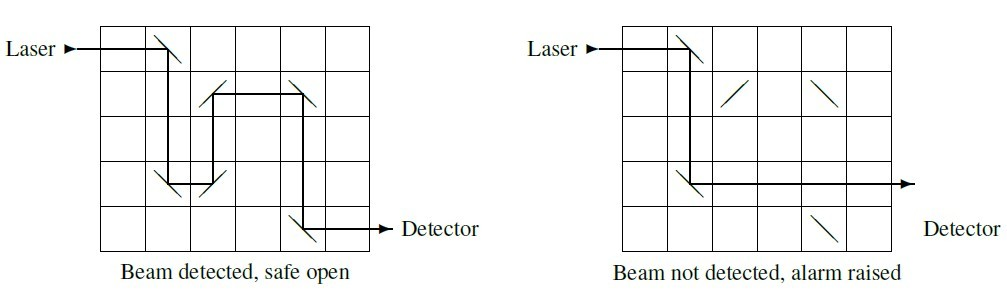
\includegraphics[width=0.8 \textwidth]{4.jpg}
					\caption{两个例子,左图能实现 1.,右图需在 $(4,3) $ 放一张 / 型镜子 才能实现 1.}
				\end{figure}
				
				$N,M \le \num{1 000 000},$ 两种镜子的数量 $p,q$ 分别 $\le \num{200 000}$
			\subsubsection{算法讨论}
				先求出从第一行左端射入的光线轨迹。方法是不断寻找在光线方向上的,且当前离光最近的镜子。具体地,可以先事先对镜子按横坐标优先和纵坐标优先分别排序,这样每行/列相邻的镜子在序列中也会相邻,直接查找当前光线所处镜子在序列中的前(后)一个元素,就是目标镜子。随后按照光线反射定律,计算光线的新方向。若光线射出网格,则退出运算。
					
				如果光线从最后一行向右射出,那么程序返回 1. 是正确的;否则从最后一行右端向左相反地射入光线,并用前述的方法计算其轨迹。只需判断两条轨迹是否有交,并求出交中的最小元素。
					
				求交的过程可转为扫描 $+$ 树状数组。两条轨迹可分为若干横线和若干纵线,那么可分别用一个的横线去交另一个的纵线。具体地,设有一条横向的扫描线从上至下扫描。那么用树状数组维护好扫描线上有哪些纵线。对于横线,则相当于在扫描线上询问区间是否非空。对于第一次非空,求出询问中最小的竖线坐标即可。根据相交的总次数即可回答 2., 3. 问。
			\subsubsection{时空复杂度}
				时间复杂度 $\mathcal{O}\left((p+q)\log(p+q) \right)$。
					
				空间复杂度 $\mathcal{O}\left(p+q\right)$。
		\newpage
		\subsection{ACM/ICPC World Finals 2012 K Stacking Plates}
			\subsubsection{题目大意}
				$N$ 碟盘堆,小盘在大盘上,可能会有相同大小的盘。请使用分割和合并盘子的方式,在保证全过程中小盘在上大盘在下的情况下,将所有盘堆合并为 1 堆。并最小化合并和分割的总次数。
			
				$N \le 50$,各个盘堆的盘子数  $M_i \le 50$。
				
				\begin{figure}[!htb]
 					\centering
					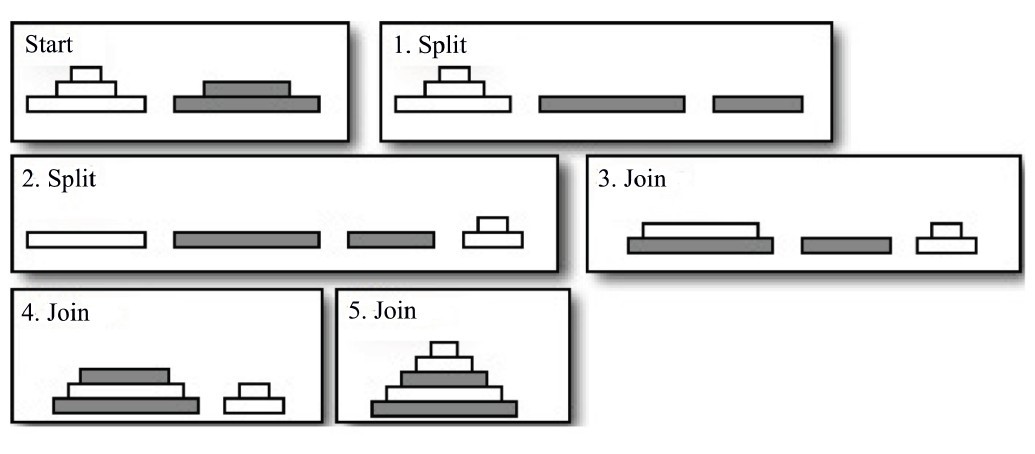
\includegraphics[width=0.8 \textwidth]{5.jpg}
					\caption{样例}
				\end{figure}
				
			\subsubsection{算法讨论}
				为处理方便,先将同一堆中相同大小的盘子合并为一个,并适当修改 $M_i$。显然答案不会被影响,因为可将被合并的看为整体来操作。
				
				由于最后需合并为一个盘堆,故不同大小的盘子的上下顺序就已经确定。只需确定相同大小间盘子的上下顺序,并求出有多少相邻盘子最开始来自于相同盘堆。设这个数为 $x$,那么分析可得答案
				\begin{align}
					Ans = 2 \sum_{i=1}^{N} M_i - N -1 -2x	
				\end{align}
				
				接下来通过动态规划确定最大的 $x$。设 $F[i][j]$ 表示已经确定好大小不超过 $i$ 的盘子的顺序,且其最底部的盘子来自堆 $j$ 的情况下,最大的 $x$。
				\begin{align}
					F[i][j]&= \max_{k} F[Last[i]][k] + [k = j], && \text{大小为  $i$ 的盘子仅存在于盘堆 $j$ }\\
					F[i][j]&= \max_{k} F[Last[i]][k] + \min_{\scriptsize p\ne j,  \atop \text{盘堆  $p$ 有大小为  $i$ 的盘子}}[k = p], && \text{ 大小为  $i$ 的盘子存在于多个盘堆}
				\end{align}边界
				\begin{align}
					F[-\infty][0]&= 0
				\end{align}可求出
				\begin{align} x &= \max_i{F[Last[+\infty]][i]}\end{align}
				其中 $Last[i]$ 表示低于 $i$ 的最大盘子大小。
				
			\subsubsection{时空复杂度}
				时间复杂度 $\mathcal{O}\left(\sum M_iN^3\right)$。使用保存最大值,优先考虑转移的方法,可去掉很多不必要的转移,将时间复杂度优化为 $\mathcal{O}\left(\sum M_iN\right)$。但对本题来说没有必要。
					
				空间复杂度 $\mathcal{O}\left(\sum M_i N\right)$。滚动优化后可降低为 $\mathcal{O}\left(N\right)$。
		\newpage